\documentclass[12pt,a4paper,titlepage]{article}
\usepackage[utf8]{inputenc}
\usepackage[finnish]{babel}
\usepackage{setspace}
\usepackage{parskip}
\usepackage{amssymb}
\usepackage{amsmath}
\usepackage{graphicx}
\usepackage{fancyhdr}
\usepackage[top=1in, bottom=1in, left=1in, right=1in]{geometry}
\usepackage{float}
\usepackage{ wasysym }

% hyödyllisiä paketteja:
\usepackage{siunitx}\sisetup{per=frac} % SI-yksiköitä.
%\usepackage{supertabular} % jos tarttee isoja taulukoita
%\usepackage{fullpage} % pienemmät marginaalit jos haluaa

\usepackage{hyperref} % lisääthän omat pakettisi ENNEN hyperref'iä
\hypersetup{pdfborder={0 0 0}}
\onehalfspacing
\cfoot{}
\rhead{\thepage}
% asettaa nyk. kappaleen nimen vasempaan ylänurkkaan, saa poistaa jos haluaa
\lhead{\leftmark}

% pythonjutut
\usepackage{color}
\usepackage{listings}
\usepackage{setspace}

\definecolor{Code}{rgb}{0,0,0}
\definecolor{Decorators}{rgb}{0.5,0.5,0.5}
\definecolor{Numbers}{rgb}{0.5,0,0}
\definecolor{MatchingBrackets}{rgb}{0.25,0.5,0.5}
\definecolor{Keywords}{rgb}{0,0,1}
\definecolor{self}{rgb}{0,0,0}
\definecolor{Strings}{rgb}{0,0.63,0}
\definecolor{Comments}{rgb}{0,0.63,1}
\definecolor{Backquotes}{rgb}{0,0,0}
\definecolor{Classname}{rgb}{0,0,0}
\definecolor{FunctionName}{rgb}{0,0,0}
\definecolor{Operators}{rgb}{0,0,0}
\definecolor{Background}{rgb}{0.98,0.98,0.98}

\lstset{
  literate={ö}{{\"o}}1
           {ä}{{\"a}}1
           {ü}{{\"u}}1
}
\lstdefinestyle{python}{
numbers=left,
numberstyle=\footnotesize,
numbersep=1em,
xleftmargin=1em,
framextopmargin=2em,
framexbottommargin=2em,
showspaces=false,
showtabs=false,
showstringspaces=false,
frame=l,
tabsize=4,
% Basic
basicstyle=\ttfamily\small\setstretch{1},
backgroundcolor=\color{Background},
language=Python,
% Comments
commentstyle=\color{Comments}\slshape,
% Strings
stringstyle=\color{Strings},
morecomment=[s][\color{Strings}]{"""}{"""},
morecomment=[s][\color{Strings}]{'''}{'''},
% keywords
morekeywords={import,from,class,def,for,while,if,is,in,elif,else,not,and,
or,print,break,continue,return,True,False,None,access,as,,del,except,exec,
finally,global,import,lambda,pass,print,raise,try,assert},
keywordstyle={\color{Keywords}\bfseries},
% additional keywords
morekeywords={[2]@invariant},
keywordstyle={[2]\color{Decorators}\slshape},
emph={self},
emphstyle={\color{self}\slshape},
breaklines=true,
breakatwhitespace=true
postbreak=\raisebox{0ex}[0ex][0ex]{\ensuremath{\color{red}\hookrightarrow\space}}
}

%%%%% kansilehti %%%%%
\title{Taivaanmekaniikka \\ Numeerinen integrointi Runge-Kutta -menetelmällä \vspace{0.5em}}
\author{\begin{tabular}{c}
Anni Järvenpää
\end{tabular}}
\date{\today}
\begin{document}
\maketitle

\newpage
\null
\thispagestyle{empty}
\addtocounter{page}{-1}
\newpage

%%%%%%%%%%%%%%% Oleellinen sisältö alkaa%%%%%%%%%%%%%%%
\section{Runge-Kutta -menetelmä} \label{menetelma}
Runge-Kutta -menetelmällä voidaan ratkaista numeerisesti differentiaaliyhtälöitä. Sitä voidaan käyttää mihin tahansa muotoa
\begin{align*}
	&y'=f(t,y) \\
	&y(t_0)=y_o
\end{align*}
olevaan alkuarvo-ongelmaan. Riippuen halutusta tarkkuudesta voidaan käyttää esimerkiksi toisen, neljännen tai kahdeksannen asteen Runge-Kutta -menetelmää. Näistä neljännen asteen menetelmä (RK4) on kuitenkin usein paras kompromissi suorituskyvyn ja tarkkuuden välillä. RK4-menetelmää käytettäessä määritellään
\begin{equation}
	y_{n+1} = y_n + \frac{h}{6}(k_1+2k_2+2k_3+k_4)
\end{equation}
missä
\begin{align*}
	k_1 &= f(t_n, y_n) \\
	k_2 &= f(t_n + \frac{h}{2}, y_n + k_1\frac{h}{2})\\
	k_3 &= f(t_n + \frac{h}{2}, y_n + k_2\frac{h}{2})\\
	k_4 &= f(t_n, y_n+k_3h)
\end{align*}
ja h on haluttu aika-askeleen pituus. Näin funktion derivaatan arvoa arvioidaan kolmessa pisteessä kutakin aika-askelta kohden, joista keskimmäistä kahdesti ($k_1$ ja $k_2$). Seuraava arvo voidaan aina laskea edellisen arvon ja aika-askeleen pituuden perusteella ja näin integroida halutun välin yli.~\cite{voesnek}

\section{RK4-menetelmän soveltaminen n kappaleen\\järjestelmään}
Tutkittaessa n kappaleen järjestelmää, tiedetään kappaleiden paikoista ja nopeuksista
\begin{align*}
	\vec{r} &=
	\begin{bmatrix}
		x \\
		y \\
		z
	\end{bmatrix}\\
	\vec{v} &=
	\begin{bmatrix}
		\dot x \\
		\dot y \\
		\dot z
	\end{bmatrix}\\
	\vec{a} &=
	\begin{bmatrix}
		\ddot x \\
		\ddot y \\
		\ddot z
	\end{bmatrix}.
\end{align*}
Näistä nähdään kappaleiden liikkeen määräävät differentiaaliyhtälöt
\begin{align*}
	\dot\vec{r} &= \vec{v}\\
	\dot\vec{v} &= \vec{a}.
\end{align*}
Järjestelmässä, jossa vaikuttaa ainoastaan painovoima, pätee
\begin{align*}
	\dot\vec{r}_i &= \vec{v}_i \\
	\dot\vec{v}_i &= \gamma \sum_{i=1}^n\sum_{j=0, j!=i}^n{m_j\frac{\vec{r}_i-\vec{r}_j}{|{r_{ij}^3}|}},
\end{align*}
missä
\begin{equation*}
	r_{ij} = |\vec r_i - \vec r_j |.
\end{equation*}
Nyt sekä paikat että nopeudet yhden aika-askeleen kuluttua saadaan, kun merkitään $f = \dot\vec{r}$ ja $g = \dot\vec{v}$ ja näille lasketaan kertoimet $k$ kummallekin funktiolle vuorotellen:
\begin{align*}
	k_{1,r} &= f(r_0, y_0)\\
	k_{1,v} &= g(r_0, y_0)\\
	k_{2,r} &= f(r_0 + \frac{1}{2}\tau k_{1,r}, v_0 + \frac{1}{2}\tau k_{1,v})\\
	k_{2,v} &= f(r_0 + \frac{1}{2}\tau k_{1,r}, v_0 + \frac{1}{2}\tau k_{1,v})\\
	k_{3,r} &= f(r_0 + \frac{1}{2}\tau k_{2,r}, v_0 + \frac{1}{2}\tau k_{2,v})\\
	k_{3,v} &= f(r_0 + \frac{1}{2}\tau k_{2,r}, v_0 + \frac{1}{2}\tau k_{2,v})\\
	k_{4,r} &= f(r_0 + \tau, v_0 + \tau)\\
	k_{4,v} &= g(r_0 + \tau, v_0 + \tau)
\end{align*}
ja näistä
\begin{align*}
	r_1 = r_0 + \frac{1}{6}\tau(k_{1,r} + 2k_{2,r} + 2k_{3,r} + k_{4,r}) \\
	v_1 = v_0 + \frac{1}{6}\tau(k_{1,v} + 2k_{2,v} + 2k_{3,v} + k_{4,v}) \\
\end{align*}
missä $\tau$ on käytetty aika-askeleen pituus.\cite{voesnek}

\section{Planeettakunnan HR 8799 simuloiminen\\RK4-menetelmällä}
Eksoplaneettakunnan HR 8799 dynaamisen evoluution tutkimiseksi toteutin oman RK4-implementaation Pythonilla. Kirjoittamani ohjelma on nähtävillä Githubissa \url{https://github.com/aajarven/runge-kutta}. Alkuarvot määritin planeettojen rataelementtien perusteella siten, että planeetat olivat simulaation alussa likimain samassa asennossa kuin kuvassa \ref{directimage}, jolloin alkuarvoiksi tuli taulukon \ref{alkuarvotaulukko} mukaiset arvot \cite{exob, exoc, exod, exoe}.

\begin{table}
	\begin{centering}
		\begin{tabular}{| l l l | l l l | l|}
			\hline
			$r_0$ (AU) & & & $v_0$ (AU/yr) & & & M ($\text{M}_{\astrosun}$)\\
			\hline
			0 & 0 & 0 & 0 & 0 & 0 & 1.56 \\
			-60.5884 & 30.8714 & 0 & -0.43205 & -0.847947 & 0 & 6.6845e-3 \\
			12.5497 & -24.8536 & 0 & 1.39023 & 0.590117 & 0 & 9.5492e-3 \\
			5.66560 & -13.3473 & 0 & 1.89707 & 0.80526 & 0 & 8.5943e-3 \\
			\hline
		\end{tabular}
		\caption{Tähden ja planeettojen paikat, nopeudet ja massat simulaation alussa.}
	\end{centering}
	\label{alkuarvotaulukko}
\end{table}

\begin{figure}
\centering
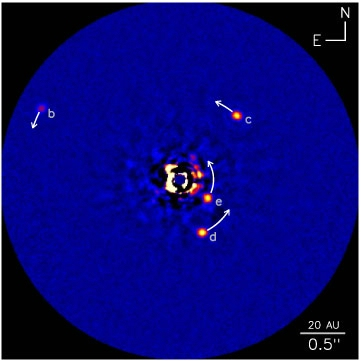
\includegraphics[width=10cm]{directimage.jpg}
\caption{W. M. Keck -teleskoopin kuva planeettakunnasta HR 8799 (Ben Zuckerman [CC BY 3.0])}
\label{directimage}
\end{figure}

Näistä loin liitteessä \ref{alkuarvot} esitetyn alkuarvotiedoston. Tiedostossa kukin kappale on omalla rivillään vektorien komponentit pilkulla eroteltuna ja vektorit puolipisteellä. \#-merkillä alkavat rivit ovat kommentteja, eikä ohjelma huomioi niitä. Lisäksi kirjoitin yksinkertaisen skriptin, jolla voidaan helposti sekä ajaa simulaatio että plotata sen tulokset yhdellä komennolla. Tämä skripti on nähtävissä liitteessä \ref{skripti}.

Liitteen \ref{alkuarvot} alkuarvoilla ajetun simulaation tuloksia on nähtävillä kuvissa \ref{10-0.001}--\ref{10000-0.01}. Kaikissa ploteissa yksikkönä on AU ja systeemin massakeskipiste on origossa. Violetilla tähti, punaisella b-, oranssilla c-, vihreällä d- ja sinisellä e-planeetta. Ploteista kahdessa ensimmäisessä ei ole nähtävissä mitään erikoista, mutta tuhannen vuoden simulaatioissa nähdään selvästi, etteivät planeettojen radat ole sulkeutuvia käyriä, vaan niissä esiintyy selvästi havaittavaa huojuntaa. Aika-askeleen lyhentäminen ei vähennä tätä efektiä, kuten kuvia \ref{1000-0.01} ja \ref{1000-0.001} vertaamalla voidaan huomata. 10 000 vuoden simulaatiossa (kuva \ref{10000-0.01}) tämä efekti on vielä selvemmin nähtävissä.

Todennäköisesti havaitut muutokset radoissa johtuvat epätarkkuuksista rataelementeissä. Kaikista kappaleista tunnettiin ainoastaan massa ja isoakselin puolikas ja näistäkin massoissa esiintyi jopa $\text{M}_{\jupiter}$ virheitä. Yhdelle planeetoista ilmoitettiin myös radan eksentrisyys, mutta ajamassani simulaatiossa kaikki planeetat lähtevät liikkeelle nopeuksilla, jotka pitäisivät ne ympyräradoilla, mikäli ne vuorovaikuttaisivat pelkästään tähden kanssa. Jonkin verran esimerkiksi Aurinkokuntaa kaoottisempi tutkittu järjestelmä saattaa kuitenkin todellisuudessakin olla, sillä planeettakunnassa on Aurinkokuntaa enemmän massiivisia planeettoja, jotka häiritsevät toisiaan.

Järjestelmän kehitystä voidaan laskea RK4-menetelmällä niin pitkälle kuin käytössä oleva laskenta-aika ja muisti sallivat. Pitkissä ajoissa lähtöarvojen tarkkuuden merkitys kuitenkin korostuu, sillä pienet häiriöt saattavat kasaantua. 

\begin{figure}
\centering
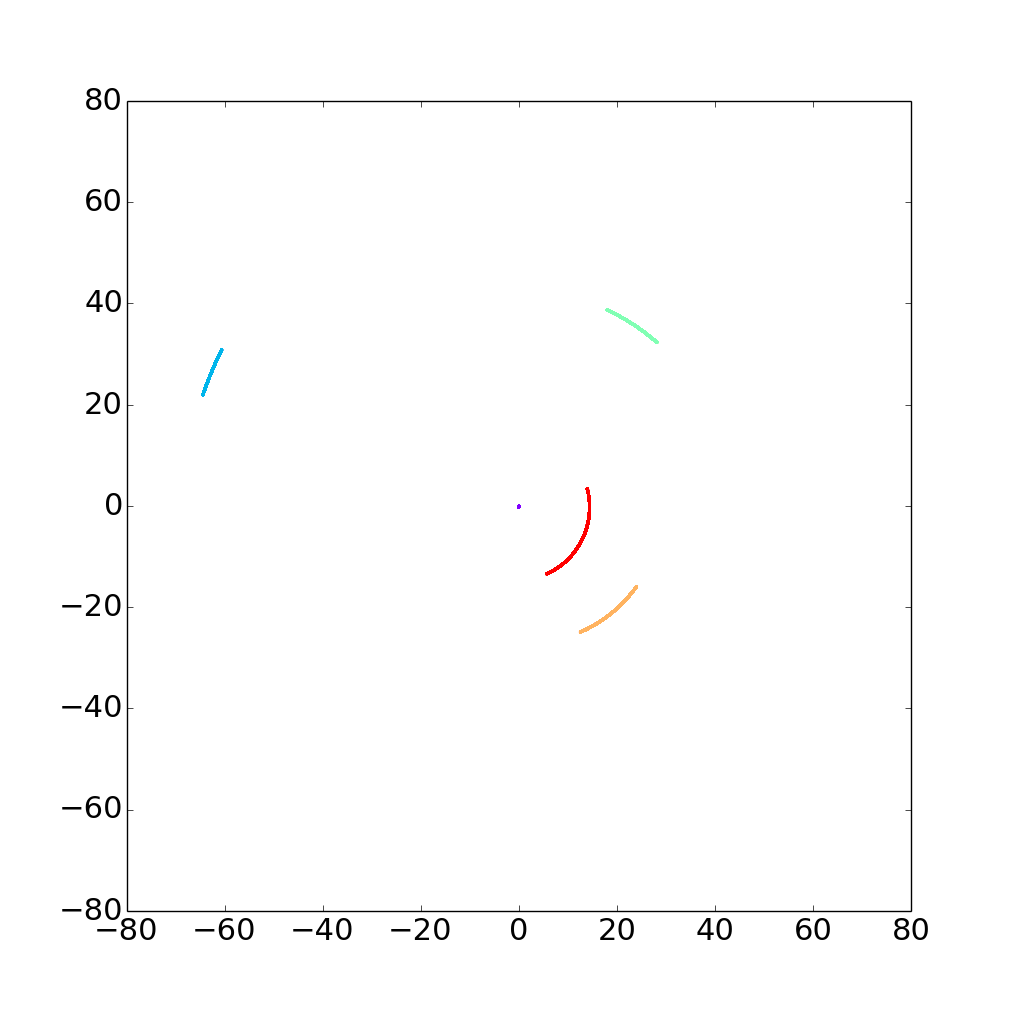
\includegraphics[width=10cm]{../kuvat/10-0001-mkp.png}
\caption{10 vuotta 0,001 vuoden (0,37 d) aika-askeleella}
\label{10-0.001}
\end{figure}

\begin{figure}
\centering
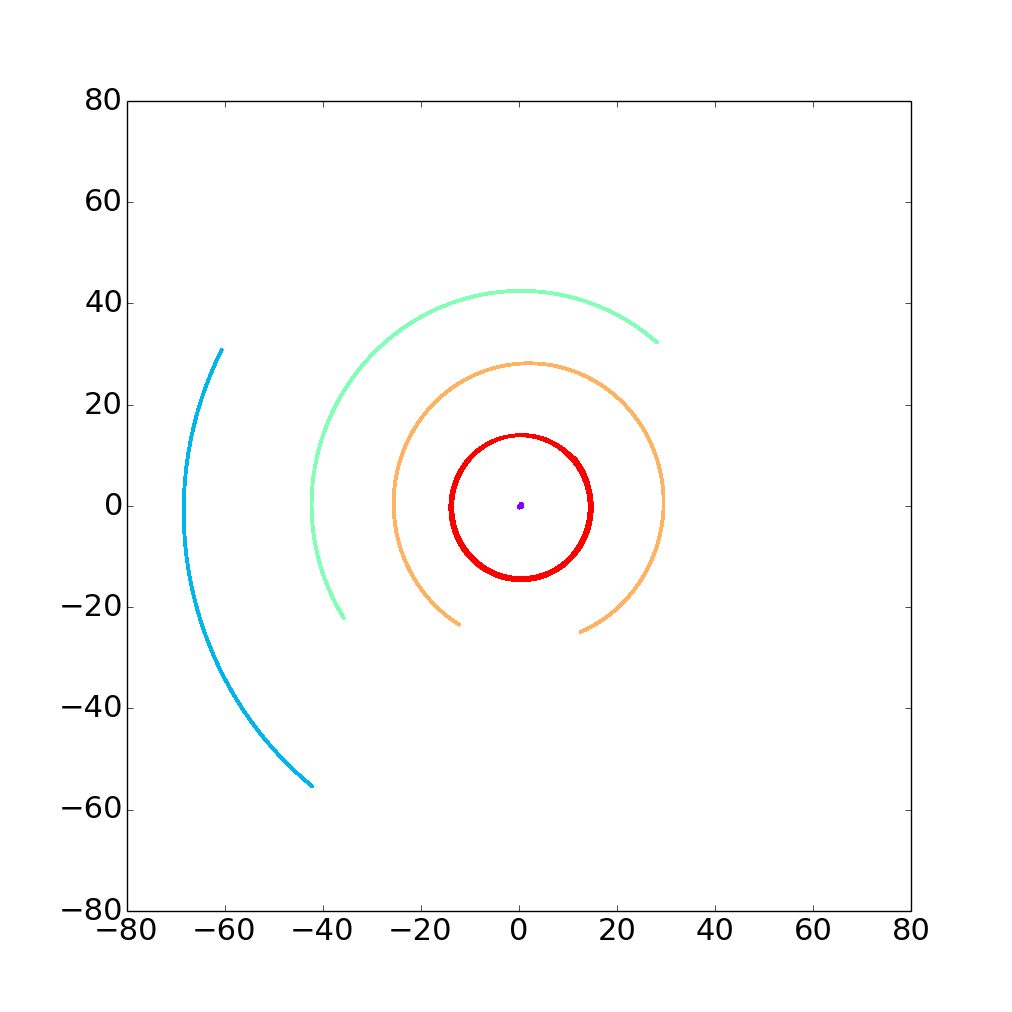
\includegraphics[width=10cm]{../kuvat/100-0001-mkp.png}
\caption{100 vuotta 0,001 vuoden (0,37 d) aika-askeleella}
\label{100-0.001}
\end{figure}

\begin{figure}
\centering
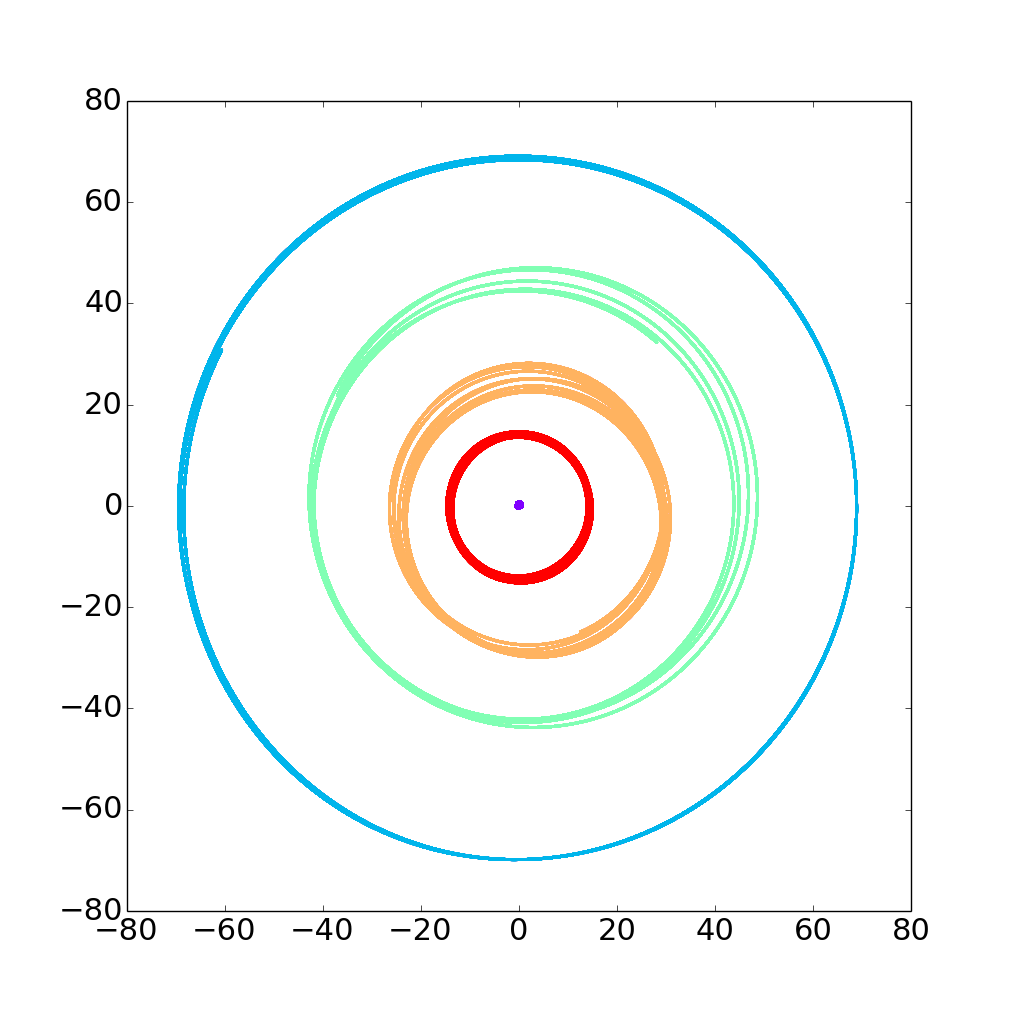
\includegraphics[width=10cm]{../kuvat/1000-001-mkp.png}
\caption{1000 vuotta 0,01 vuoden (3,7 d) aika-askeleella}
\label{1000-0.01}
\end{figure}

\begin{figure}
\centering
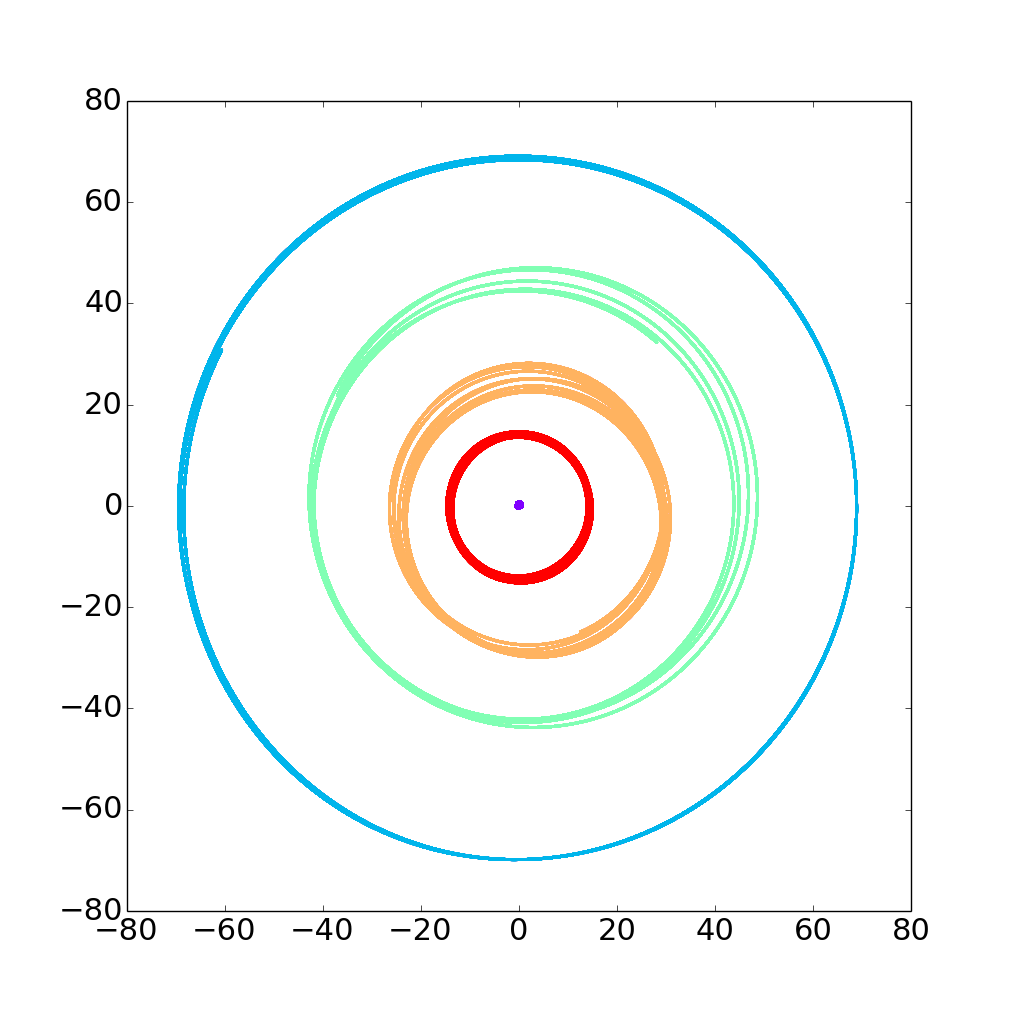
\includegraphics[width=10cm]{../kuvat/1000-001-mkp.png}
\caption{1000 vuotta 0,001 vuoden (0,37 d) aika-askeleella}
\label{1000-0.001}
\end{figure}

\begin{figure}
\centering
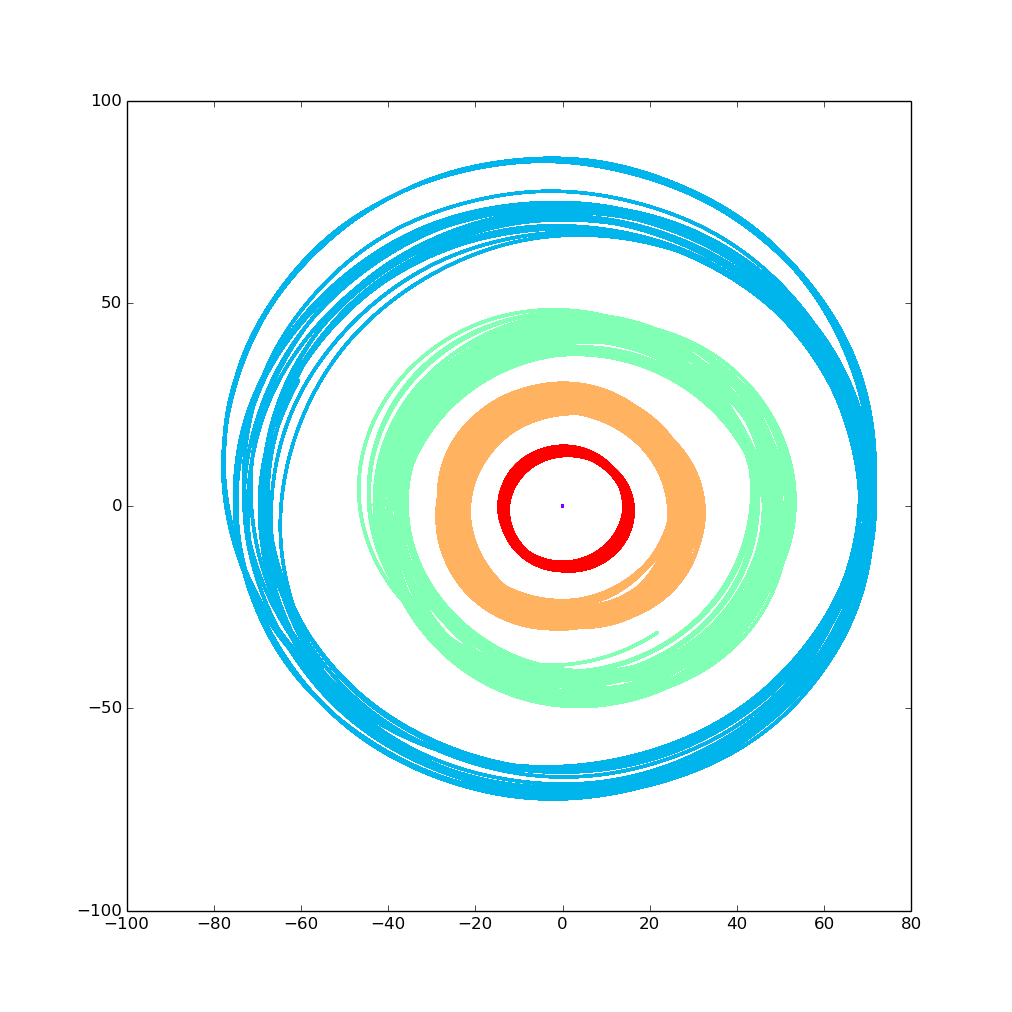
\includegraphics[width=10cm]{../kuvat/10000-001.png}
\caption{10000 vuotta 0,01 vuoden (3,7 d) aika-askeleella}
\label{10000-0.01}
\end{figure}

%%%%% Sisältö loppuu, lähdeluettelo %%%%%
\newpage
\bibliographystyle{plain}
\bibliography{lahteet} 
\appendix
\newpage
\section{Käytetty alkuarvotiedosto} \label{alkuarvot}
\lstinputlisting[basicstyle=\ttfamily]{hr8799.txt}
\newpage
\section{Simulointi- ja plottausskripti} \label{skripti}
\lstinputlisting[basicstyle=\ttfamily,language=bash,showstringspaces=false,breaklines=true]{skripti.txt}
\newpage
\end{document}
